\documentclass[tikz]{standalone}
\usetikzlibrary{shapes}
\begin{document}
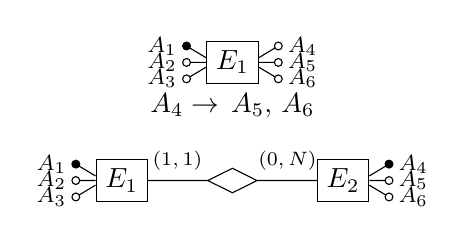
\begin{tikzpicture}
    \draw

    %%* Attributi:
    %%  node[draw, circle, inner sep=1pt, fill=black]{}node[right]{\footnotesize A}
    %%? Distanza orizzontale: E -(0.25,0.x)- A
    %%? Distanza verticale: E -(0,x * 0.22)- A

    %%* Cardinalità:
    %%  node[below right]{\scriptsize $(0,N)$}
    %%  node[above right]{\scriptsize $(0,N)$}
    %%  node[midway, above]{\scriptsize $(0,N)$}

    %%* Relazione:
    %%  node[draw, diamond, shape aspect=2, inner sep=3pt, anchor=90](r1){}
    %%  node[draw, diamond, shape aspect=2, inner sep=0.2pt, anchor=180](r2){R2}

    %%* Entità:
    %%  node[draw, rectangle, anchor=90](e1){}
    %%? Distanza verticale: E -(0.3)- R -(0.3) E
    %%? Distanza orizzontale: E -(0.75)- R -(0.75)- E

    (0,0)node[draw, rectangle,label=below:{$A_4\to\,A_5,\,A_6$}](e1){$E_1$}

    (e1.190)--++(-0.25,-0.15)node[draw, circle, inner sep=1pt, fill=white]{}node[left]{\footnotesize $A_3$}
    (e1.180)--++(-0.25,0)node[draw, circle, inner sep=1pt, fill=white]{}node[left]{\footnotesize $A_2$}
    (e1.170)--++(-0.25,0.15) node[draw, circle, inner sep=1pt, fill=black]{}node[left]{\footnotesize $A_1$}

    (e1.350)--++(0.25,-0.15)node[draw, circle, inner sep=1pt, fill=white]{}node[right]{\footnotesize $A_6$}
    (e1.0)--++(0.25,0)node[draw, circle, inner sep=1pt, fill=white]{}node[right]{\footnotesize $A_5$}
    (e1.10)--++(0.25,0.15) node[draw, circle, inner sep=1pt, fill=white]{}node[right]{\footnotesize $A_4$}



    (0,-1.5)node[draw, diamond, shape aspect=2, inner sep=3pt](r1){}
    (r1.180)--++(-0.75,0)node[midway, above]{\scriptsize $(1,1)$}node[draw, rectangle, anchor=0](e1){$E_1$}
    (e1.190)--++(-0.25,-0.15)node[draw, circle, inner sep=1pt, fill=white]{}node[left]{\footnotesize $A_3$}
    (e1.180)--++(-0.25,0)node[draw, circle, inner sep=1pt, fill=white]{}node[left]{\footnotesize $A_2$}
    (e1.170)--++(-0.25,0.15) node[draw, circle, inner sep=1pt, fill=black]{}node[left]{\footnotesize $A_1$}
    (r1.0)--++(0.75,0)node[midway, above]{\scriptsize $(0,N)$}node[draw, rectangle, anchor=180](e1){$E_2$}
    (e1.350)--++(0.25,-0.15)node[draw, circle, inner sep=1pt, fill=white]{}node[right]{\footnotesize $A_6$}
    (e1.0)--++(0.25,0)node[draw, circle, inner sep=1pt, fill=white]{}node[right]{\footnotesize $A_5$}
    (e1.10)--++(0.25,0.15) node[draw, circle, inner sep=1pt, fill=black]{}node[right]{\footnotesize $A_4$}

    ;
\end{tikzpicture}
\end{document}